\documentclass{article}

\usepackage{color}
\usepackage{graphicx}
\usepackage{tabularx}


\usepackage{geometry,wrapfig,lipsum}
 \geometry{
 top=20mm,
 bottom=20mm,
 }


\title{Hacking}
\author{Justal Kevin}
\date{30/10/2015}
\renewcommand{\contentsname}{Table des mati\`eres} 
 
\newcommand\invisiblesection[1]{%
  \refstepcounter{section}%
  \addcontentsline{toc}{section}{\protect\numberline{\thesection}#1}%
  \sectionmark{#1}} 
 
\begin{document}

\begin{center}
\textbf{\Huge{FAILLE WEB}}
\line(1,0){300}\\
Verrou par verrou et l'un apr\`es l'autre, aucun syst\`eme ne r\'esistera !\\
\vspace{3cm}

\includegraphics[width=\textwidth]{0}\\
\vspace{3cm}
\textbf{\Large{JUSTAL KEVIN}}\\
2014-2015\\
\vspace{4cm}
\textbf{Justal Kevin - \color{blue}{\underline{justal.kevin@gmail.com}}}\\
\end{center}

\newpage
\tableofcontents

\newpage
\section{Directory transversal - Attaque sur le htaccess}
\subsection{Explications}
\subsubsection{Qu'est ce que la technologie htaccess ?}
\hspace*{0.6cm}Les fichiers .htaccess sont des fichiers de configuration de Apache. Ils permettent de s\'ecuris\'e via un mot de passe et un identifiant l'acc\'es \`a une zone du serveur. Ils sont localis\'es et ne peuvent affecter que les r\'epertoire o\`u ils r\'esident. La particularit\'e d'une telle fonctionnalit\'e apporte deux avantages. D'une part, on peux d\'el\'eguer la gestion d'une partie du site sans donner le droit de g\'erer le serveur lui-m\^eme. D'autre part, les modifications sont prises en compte sans qu'il soit n\'ecessaire de red\'emarrer le serveur HTML.

\subsubsection{Les directives htaccess}
\hspace*{0.6cm}Un fichier htaccess prend la forme suivante :
\vspace{0.2cm}\\
\fbox{\parbox{\textwidth}{
\hspace*{0.6cm}AuthUserFile /var/www/.htpasswd\\
\hspace*{0.6cm}AuthName "Visiteur, vous pénétrez dans une section réservée aux membres, veuillez vous identifier"\\
\hspace*{0.6cm}AuthType Basic\\
\hspace*{0.6cm}require Admin
}}
\vspace{0.2cm}\\
\hspace*{0.6cm}La premi\`ere directive, \textbf{AuthUserFile}, est le lien entre le htaccess et le htpasswd. Cette simple directive indique simplement o\`u se situe le fichier htpasswd. Le chemin inscrit ici est g\'en\'eralement le chemin d'acc\`es absolue mais il est possible de trouver aussi un chemin relative mais cela reste tout de m\^eme relativement rare.
\vspace{0.2cm}\\
La directive \textbf{AuthName} permet de sp\'ecifier un titre \`a la fen\^etre de connexion.
\vspace{0.2cm}\\
\hspace*{0.6cm}La directive \textbf{AuthType} indique le type d'authentification. Il n'existe que deux types possibles : Basic ou Digest. Le premier type indique simplement que le mot de passe lors de l'authentification sera transmise en clair du client au serveur. C'est pourquoi cette m\'ethode n'est pas \`a utiliser pour un transfert de donn\'ee sensible. Le type Digest est un sois-disant type am\'eliorant la s\'ecurit\'e du transfert, cependant de nombreuses failles existent ici. Ce qui rend ce type inutile car plus lourd \`a mettre en place et pas vraiment s\'ecuris\'e.
\vspace{0.2cm}\\
La directive \textbf{requiere} sp\'ecifie simplement qui est autoris\'e \`a acc\'eder \`a cette partie du site. On ira donc chercher dans le fichier htpasswd l'utilisateur Admin pour comparer le mot de passe.
\subsubsection{Les directives htpasswd}
\hspace*{0.6cm}Un fichier htpasswd prend la forme suivante :
\vspace{0.2cm}\\
\fbox{\parbox{\textwidth}{
\hspace*{0.6cm}admin1:\$apr1\$Ikl22aeJ\$w1uWlBGlbatPnETT2XGx.. \\
\hspace*{0.6cm}admin2:\$apr1\$yJnQGpTi\$WF5eCC/8lKsgBKY7fvag60 
}}
\vspace{0.2cm}\\
\hspace*{0.6cm}Un fichier httpasswd prend toujours la forme ci-dessus. Ce fichier lie un utilisateur \`a un password crypt\'e via un algorithme comme SHA, DES, MD5...

\newpage
\subsection{La navigation transversale ou Directory transversal}
\hspace*{0.6cm}Pour expliqu\'e la faille, je prendrais un exemple. Le site w3challs.com dispose d'un exemple sur cette faille du syst\`eme. Avant m\^eme de commencer l'exp\'erimentation, il faut encore un peu d'explication pour comprendre la faille. Cette faille r\'eside dans le PHP du site et en particulier dans la balise include.
\vspace{0.2cm}\\
\fbox{\parbox{\textwidth}{
\hspace*{0.6cm}\$template = 'red.php';\\
\hspace*{0.6cm}if (isset(\$\_COOKIE['TEMPLATE']))\\
\hspace*{1.2cm}\$template = \$\_COOKIE['TEMPLATE'];\\
\hspace*{0.6cm}include ("/home/users/phpguru/templates/" . \$template);
}}
\vspace{0.2cm}\\
\hspace*{0.6cm}Ici, le fait que dans l'include, on ne v\'erifie pas que le r\'esultat attendu soit une page .html ou .php, on peux alors imaginer de modifi\'e la variable \$template. Il y a plusieurs mani\`eres de proc\'ed\'e qui d\'ependent de la mani\`ere dont est impl\'ement\'e le code du site que l'on souhaite attaquer : Par l'URL, Par la requ\`ete HTML...\\
\hspace*{0.6cm}Dans le cas ci-dessus, on utilise \$\_COOKIE, on en retient donc que la page ou la destination vers o\`u pointe \$template a \'et\'e enregistr\'e sur l'ordinateur de l'utilisateur. Il est donc possible de modifier la requ\`ete avant de l'envoyer au serveur.
\vspace{0.2cm}\\
Imaginons alors que la variable template soit "../../../.htaccess", on remonte alors les repertoires jusqu'au root. Si le systeme de la machine est Linux, il existe alors forcement un repertoire etc/passwd. Maintenant, sur les serveur en ligne, les developpeurs posent g\'en\'eralement ces dossiers dans des repertoires comme admin/.htaccess ou encore pass/.htaccess. Il suffit de faire preuve d'un peu d'imagination pour trouver o\`u pourrait se trouver le fichier.

\subsection{Exploitation}
\hspace*{0.6cm}Sur w3chall.com, on trouve une page avec cette faille. La premi\`ere chose \`a faire est donc de chercher le fichier .htaccess. En forcant, on trouve que le fichier assez rapidement. Dans la barre d'adresse, il suffit de finir l'adresse par :
\vspace{0.2cm}\\
\fbox{\parbox{\textwidth}{
\hspace*{0.6cm}/?page=../admin/.htaccess
}}
\vspace{0.2cm}\\
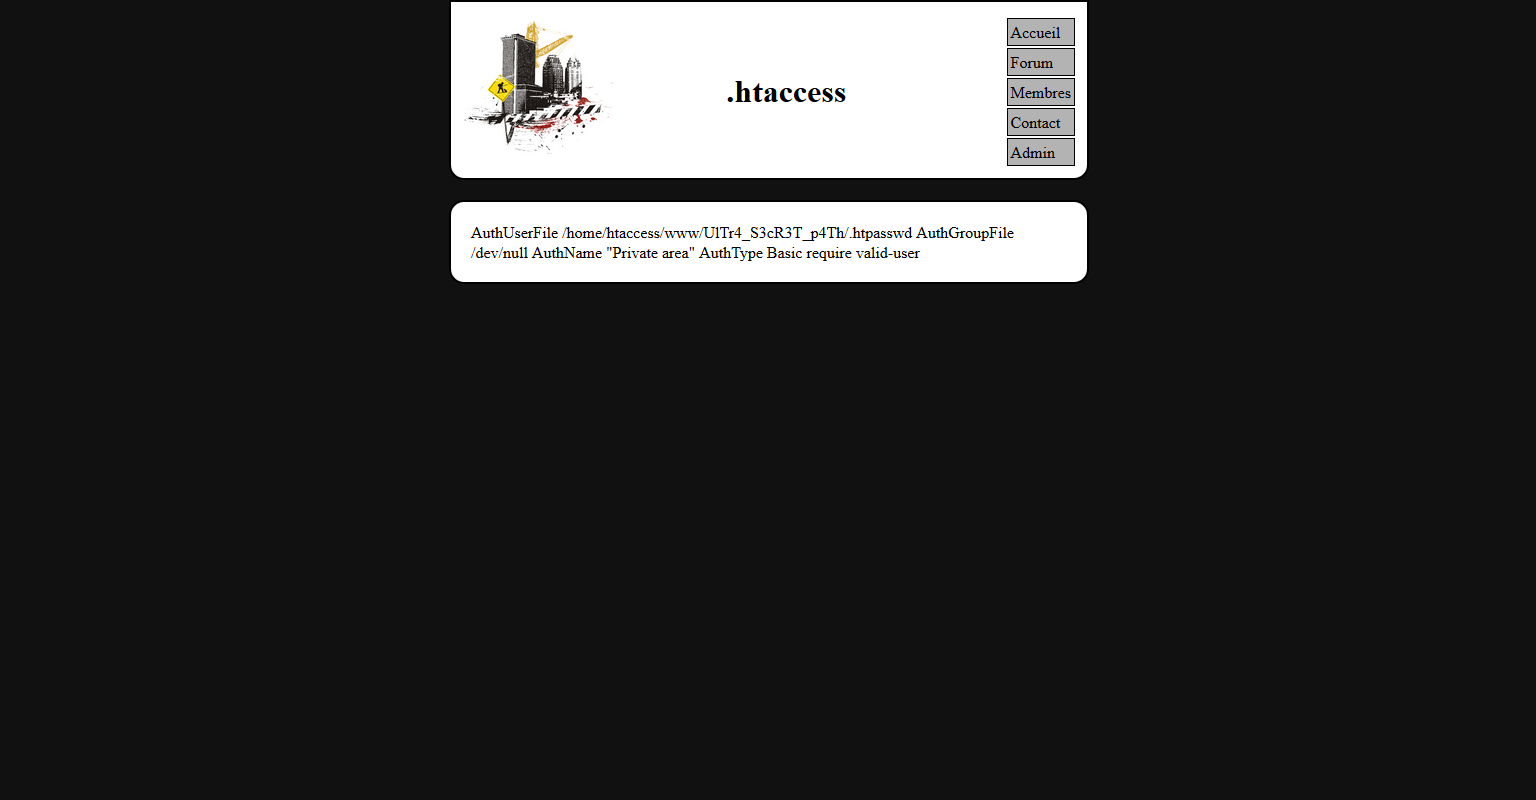
\includegraphics[width=\textwidth]{2}\\
\vspace{0.2cm}\\
Bien entendu, avant d'arriver \`a cela, j'ai tap\'e plusieurs autres chemins comme ./admin/.htaccess ou encore .htaccess. Une fois ici, on remarque la g\'en\'erosit\'e du syst\`eme qui nous donne l'emplacement exacte du fichier htpasswd. Il suffit alors de s'y rendre :
\vspace{0.2cm}\\
\fbox{\parbox{\textwidth}{
\hspace*{0.6cm}?page=../UlTr4\_S3cR3T\_p4Th/.htpasswd
}}
\vspace{0.2cm}\\
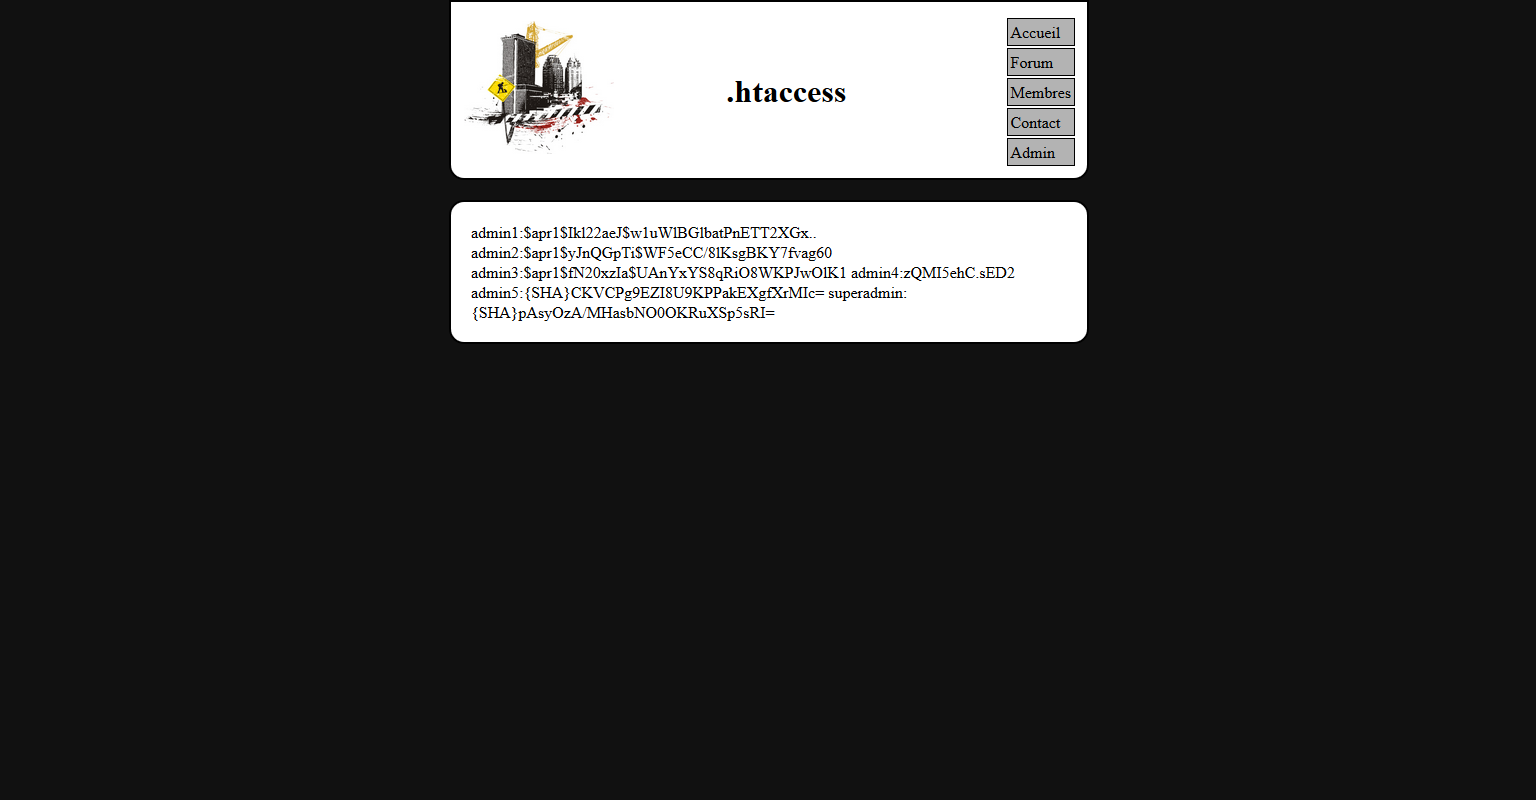
\includegraphics[width=\textwidth]{3}\\
\vspace{0.2cm}\\
\hspace*{0.6cm}Et voila qu'apparaisent sous vos yeux les passwords et logins qui se trouvent dans le fichier htpasswd. Ils sont bien entendu crypté mais avec l'utilisation d'un logiciel tiers comme John the Ripper, la reconstitution du password d'origine n'est qu'une question de temps.
\subsection{Variante}
\hspace*{0.6cm}La premi\`ere correstion apport\'e par les d\'eveloppeurs furent d'ajouter l'extension du fichier \`a la fin de l'include. Ce qui donnait un lien finissant toujours par .html ou .php. Il devient alors th\'eoriquement impossible de rentrer quelques choses finissant par aucune extension comme nous l'avons fait jusqu'\`a maintenant. Erreur ! Il est possible de terminer une chaine \`a l'endroit o\`u l'on souhaite en ajoutant le charat\`ere de fin de chaine : le null ou encore \%00. Ce qui dans notre cas donnerais :
\vspace{0.2cm}\\
\fbox{\parbox{\textwidth}{
\hspace*{0.6cm}/?page=../admin/.htaccess\%00.html
}}
\vspace{0cm}\\
Cependant le serveur ne lira cette chaine que jusqu'au charatere null, le reste sera ignor\'e.
\subsection{Solution}
Pour se pr\'emunir d'une telle attaque, pourquoi ne pas simplement escape tout les ../ ou \%2e\%2e/ (si encod\'e) lors des navigations.
\end{document}
